% https://www.javatpoint.com/linear-regression-in-machine-learning
% https://www.javatpoint.com/simple-linear-regression-in-machine-learning
% https://www.javatpoint.com/machine-learning-polynomial-regression

% https://www.javatpoint.com/k-nearest-neighbor-algorithm-for-machine-learning
% https://www.javatpoint.com/machine-learning-support-vector-machine-algorithm
% https://www.javatpoint.com/linear-regression-vs-logistic-regression-in-machine-learning
% https://www.javatpoint.com/linear-regression-in-tensorflow

\section[Conclusione]{Conclusione}
%\sectionframe{images/covers/cover_first_simple_algoritms.jpg}{Apprendimento\\supervisionato:\\i primi semplici algoritmi}

\begin{frame}
	\begin{tabular}{*{4}{c}} 
	  & \textbf{Unsupervised} & \textbf{Supervised} & \\
	  \multirow{3}*{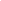
\includegraphics[width=.075\textwidth]{images/empty.png}} &   \begin{tikzpicture} \draw (0, 0) node[inner sep=0] {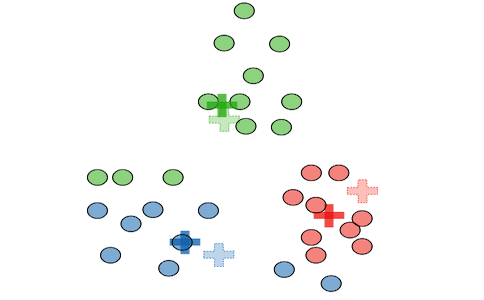
\includegraphics[width=.35\textwidth]{images/summary/kmeans.png}}; \draw (1, 1) node {K-Means};\end{tikzpicture} & \begin{tikzpicture} \draw (0, 0) node[inner sep=0] {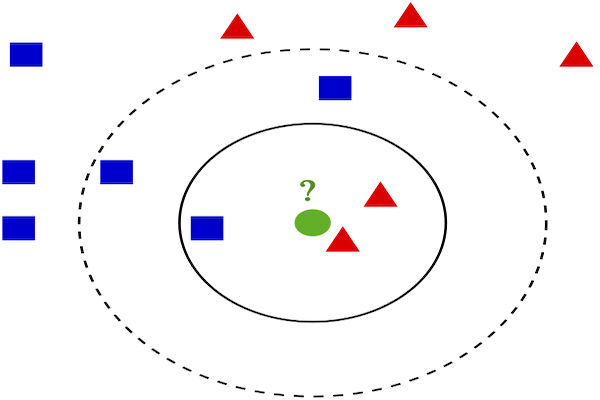
\includegraphics[width=.35\textwidth]{images/summary/knn.png}}; \draw (1, 1) node {KNN};\end{tikzpicture} & \multirow{3}*{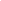
\includegraphics[width=.075\textwidth]{images/empty.png}}\\ 
	  & \begin{tikzpicture} \draw (0, 0) node[inner sep=0] {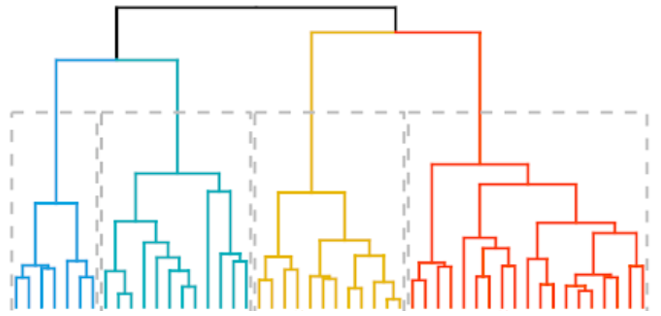
\includegraphics[width=.35\textwidth]{images/summary/hierarchical.png}}; \draw (1, 1) node {Hierarchical};\end{tikzpicture} & \begin{tikzpicture} \draw (0, 0) node[inner sep=0] {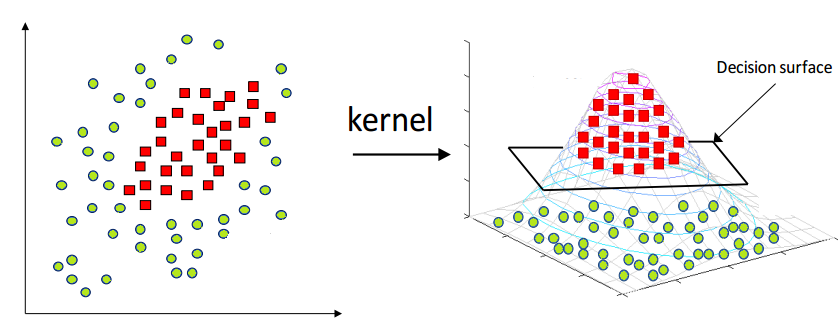
\includegraphics[width=.35\textwidth]{images/summary/perceptron.png}}; \draw (1, 1) node {Perceptron};\end{tikzpicture} & \\
	  & \begin{tikzpicture} \draw (0, 0) node[inner sep=0] {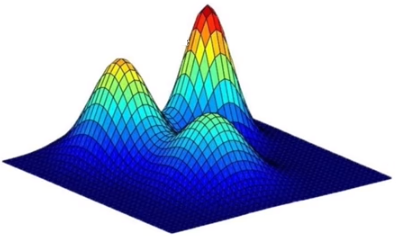
\includegraphics[width=.35\textwidth]{images/summary/gmm.png}}; \draw (1, 1) node {GMM};\end{tikzpicture} & \begin{tikzpicture} \draw (0, 0) node[inner sep=0] {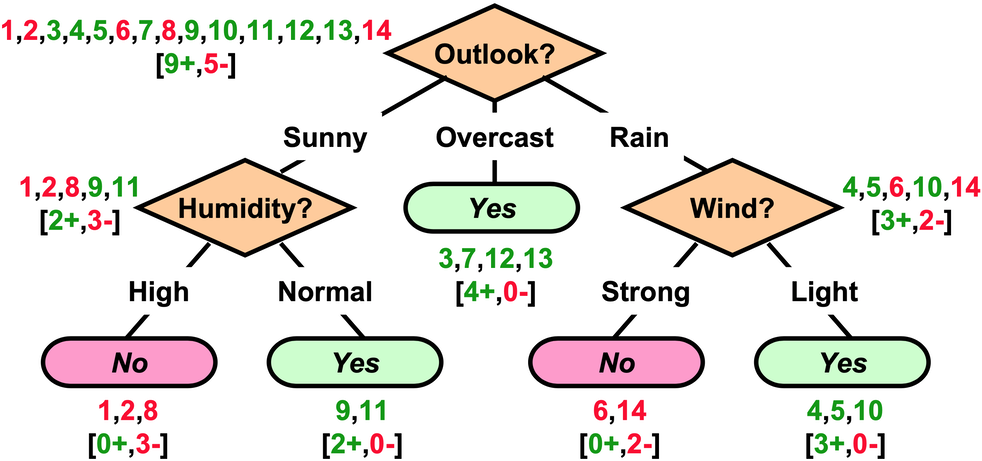
\includegraphics[width=.35\textwidth]{images/summary/id3.png}}; \draw (1, 1) node {ID3};\end{tikzpicture} & \\
	\end{tabular}
\end{frame}